\documentclass{article}
\usepackage[utf8]{inputenc}
\usepackage[siunitx]{circuitikz}
\usepackage{amsmath}
\usepackage{graphicx}
\usepackage[a4paper, total={6in, 8in}]{geometry}

\title{Hardverski interfejsi - domaći zadatak}
\author{Nenad Radović, RA18/2020}
\date{18. mart, 2023. godina}

\begin{document}

    \maketitle

    \section{Problem i prijedlog rješenja}

    \begin{figure}[h]

        \centering

        \begin{circuitikz}
            
            \draw
            (0, 3) node[label=west:$v_{in}(t)$] {}
            (0, 3) to[nos, o-, i=$i_1(t)$] (3, 3)
            (3, 3) to[R, l=$R_1$, v<=$v_1(t)$, -*] (6, 3)
            (6, 3) to[R, l=$R_2$, v<=$v_2(t)$, i=$i_2(t)$] (6, 0)
            (6, 0) node[ground]{}
            (6, 3) -- (9, 3)
            (9, 3) to[C, l=$C$, v<=$v_{out}(t)$, i=$i_3(t)$] (9, 0)
            (9, 0) node[ground]{};

        \end{circuitikz}

        \caption{Slika problema}
    
    \end{figure}

    Na slici iznad, pored obilježenog \textbf{ulaznog napona} $v_{in}(t)$ i \textbf{izlaznog napona} $v_{out}(t)$, 
    obilježimo padove napona na otpornicima $R_1$ i $R_2$ $v_1(t)$ i $v_2(t)$, respektivno.
    Takodje, obilježimo struje $i_1(t)$, $i_2(t)$ i $i_3(t)$ odabranim smjerovima, kao na slici.

    Primjetimo da je traženi izlazni napon napon na kondenzatoru. Dakle, uvidjamo vezu struje koja
    protiče kroz dati kondenzator i izlaznog napona preko jednačine

    \begin{equation}
        i_3(t) = C\frac{dv_{out}(t)}{dt}\label{eq1}
    \end{equation}

    
    Kako imamo dvije konture u kolu, primjenom Kirhofovih zakona na date dobijamo sledeći sistem jednačina:

    \begin{align}
        v_{in}(t) - R_1i_1(t) - R_2i_2(t) = 0\label{eq2} \\ 
        -v_{out}(t) + R_2i_2(t) = 0\label{eq3} \\
        i_1(t) - i_2(t) - i_3(t) = 0\label{eq4}
    \end{align}

    Izrazimo struju $i_1(t)$ iz jednačine (\ref{eq2}):

    \begin{equation}
        i_1(t) = \frac{v_{in}(t) - R_2i_2(t)}{R_1}\label{eq5}
    \end{equation}


    Primjetimo da je proizvod $R_2i_2(t)$ jednak izlaznom naponu $v_{out}(t)$ (ishodi iz jednačine
    (\ref{eq3})), tako da jednačina (\ref{eq5}) postaje:

    \begin{equation}
        i_1(t) = \frac{v_{in}(t) - v_{out}(t)}{R_1}\label{eq6}
    \end{equation}


    Pomoću strujnog Kirhofovog zakona (jednačine (\ref{eq4})), jednačinu (\ref{eq1}) možemo zapisati kao:

    \begin{equation}
        i_1(t) - i_2(t) = C\frac{dv_{out}(t)}{dt}\label{eq7}
    \end{equation}


    Preostali korak u vremenskom domenu će biti da zamijenimo prethodno dobijene izraze za struje
    $i_1(t)$ i $i_2(t)$ (jednačine (\ref{eq3}) i (\ref{eq6})) u jednačinu (\ref{eq7}):

    \begin{equation}
        \begin{split}
            C\frac{dv_{out}(t)}{dt} = \frac{v_{in}(t) - v_{out}(t)}{R_1} - \frac{v_{out}(t)}{R_2} \\
            \frac{dv_{out}(t)}{dt} = \frac{v_{in}(t)}{R_1C} - \frac{1}{C}(\frac{1}{R_1}+\frac{1}{R_2})v_{out}(t) \\
            \frac{dv_{out}(t)}{dt} + \frac{1}{C}(\frac{1}{R_1}+\frac{1}{R_2})v_{out}(t) = \frac{v_{in}(t)}{R_1C}
        \end{split}
        \label{eq8}
    \end{equation}


    Dobijamo linearnu nehomogenu diferencijalnu jednačinu konstantnih koeficijenata koju ćemo riješiti
    primjenom Laplasove transformacije.


    Dakle, iz jednačine (\ref{eq8}) i primjenom Laplasove transformacije, slijedi da je:

    \begin{equation}
        sV_{out}(s) - v_{out}(0^-) + \frac{1}{C}(\frac{1}{R_1}+\frac{1}{R_2})V_{out}(s) = \frac{V_{in}(s)}{R_1C}
        \label{eq9}
    \end{equation}

    za koju važi da su $V_{in}(s)$ i $V_{out}(s)$ kompleksni predstavnici napona $v_{in}(t)$ i $v_{out}(t)$, respektivno.

    Sredjivanjem izraza (\ref{eq9}), dobijamo funkciju prenosa od $V_{in}(s)$ ka $V_{out}(s)$:

    \begin{equation}
        V_{out}(s) = \frac{\frac{1}{R_1C}}{s+\frac{1}{C}(\frac{1}{R_1} + \frac{1}{R_2})}V_{in}(s) + \frac{1}{s+\frac{1}{C}(\frac{1}{R_1} + \frac{1}{R_2})}v_{out}(0^-)
        \label{eq10}
    \end{equation}

    Pretpostavimo da je u početnom trenutku kondenzator prazan. Tada će važiti da $v_{out}(0^-) = 0 $,
    te se time anulira desni sabirak desne strane jednačine (\ref{eq10}).

    Po postavci zadatka, u trenutku $t = 0$ prekidač je zatvoren i u tom je stanju sve do trenutka $t = 7$,
    kada se otvara. Takvo ponašanje možemo modelovati zbirom Hevisajdovih step funkcija $v_{in}(t) = h(t) - h(t - 7)$. 
    Time dobijamo da je kompleksni predstavnik $V_{in}(s)$ jednak $\frac{1}{s} - \frac{1}{s}e^{-7s}$

    Slijedi da važi:

    \begin{equation}
        V_{out}(s) = \frac{\frac{1}{R_1C}}{s+\frac{1}{C}(\frac{1}{R_1} + \frac{1}{R_2})}(\frac{1}{s} - \frac{1}{s}e^{-7s})
    \end{equation}


    Izraz za $V_{out}(s)$ možemo srediti rastavljanjem na parcijalne razlomke. Postupak je sledeći:

    \begin{equation}
        \begin{split}
            \frac{\frac{1}{R_1C}}{s(s + \frac{1}{C}(\frac{1}{R_1} + \frac{1}{R_2}))} = \frac{A}{s} + \frac{B}{s + \frac{1}{C}(\frac{1}{R_1} + \frac{1}{R_2})} \\
            \frac{\frac{1}{R_1C}}{s(s + \frac{1}{C}(\frac{1}{R_1} + \frac{1}{R_2}))} = \frac{A(s + \frac{1}{C}(\frac{1}{R_1} + \frac{1}{R_2})) + Bs}{s(s + \frac{1}{C}(\frac{1}{R_1} + \frac{1}{R_2}))} 
        \end{split}
    \end{equation}

    Dobijamo dati sistem jednačina:

    \begin{equation}
        \begin{split}
            A + B = 0 \\
            \frac{A}{C}(\frac{1}{R_1} + \frac{1}{R_2}) = \frac{1}{R_1C}
        \end{split}
    \end{equation}

    Rješenje sistema po koeficijentima $A$ i $B$ je:

    \begin{equation}
        \begin{split}
            A = \frac{R_2}{R_1 + R_2} \\
            B = -\frac{R_2}{R_1 + R_2}
        \end{split}
    \end{equation}

    Time, finalni izraz u kompleksnom domenu za izlazni napon $V_{out}(s)$ jeste:

    \begin{equation}
        \begin{split}
            V_{out}(s) = \left(\frac{\frac{R_2}{R_1 + R_2}}{s} - \frac{\frac{R_2}{R_1 + R_2}}{s + \frac{1}{C}(\frac{1}{R_1} + \frac{1}{R_2})}\right)(1 - e^{-7s}) \\
            V_{out}(s) = \frac{\frac{R_2}{R_1 + R_2}}{s} - \frac{\frac{R_2}{R_1 + R_2}}{s}e^{-7s} - \frac{\frac{R_2}{R_1 + R_2}}{s + \frac{1}{C}(\frac{1}{R_1} + \frac{1}{R_2})} + \frac{\frac{R_2}{R_1 + R_2}}{s + \frac{1}{C}(\frac{1}{R_1} + \frac{1}{R_2})}e^{-7s}
        \end{split}
    \end{equation}


    Primjenjivajući inverznu Laplasovu transformaciju na svaki od članova, dobijamo izraz za izlazni napon u vremenskom domenu:

    \begin{equation}
        v_{out}(t) = \frac{R_2}{R_1 + R_2}h(t)\left(1 - e^{-\frac{1}{C}(\frac{1}{R_1} + \frac{1}{R_2})t}\right) + \frac{R_2}{R_1 + R_2}h(t-7)\left(e^{-\frac{1}{C}(\frac{1}{R_1} + \frac{1}{R_2})(t-7)} - 1\right)
    \end{equation}

    Grafički predstavljeno, pobuda $v_{in}(t)$ i odziv $v_{out}(t)$ izgledaju:
    
    \begin{figure}[h]   
        \centering
        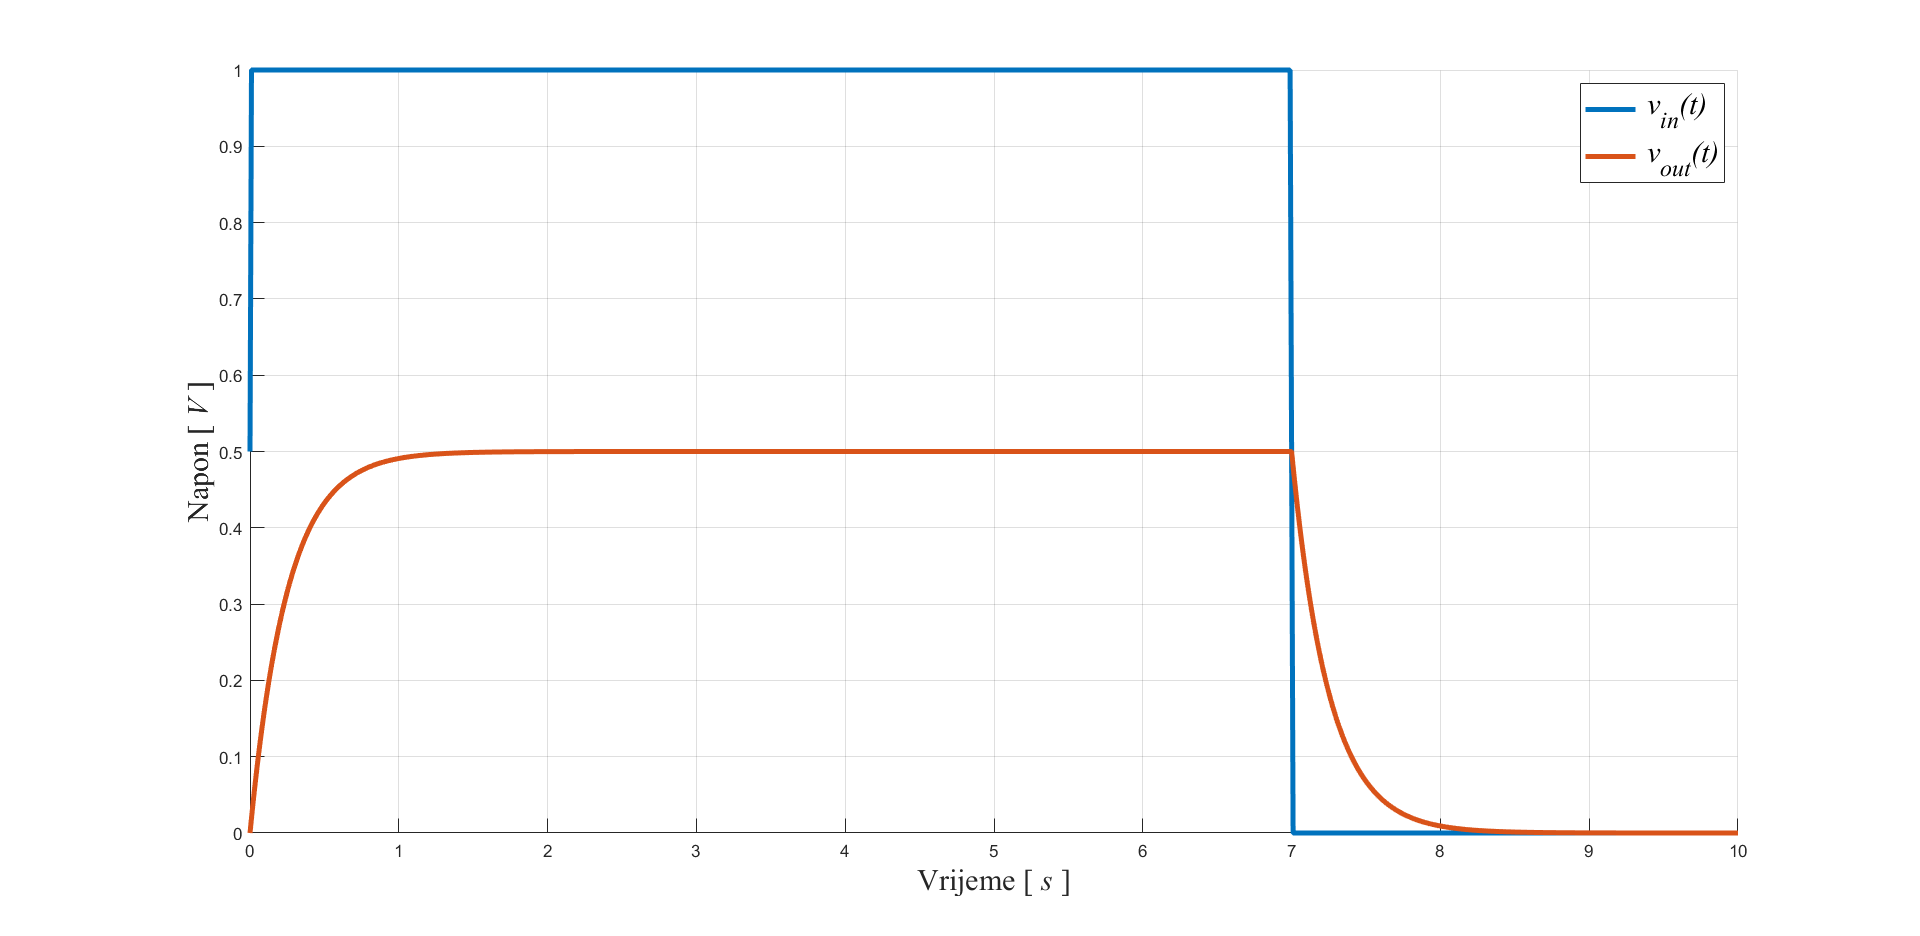
\includegraphics[width=0.85\textwidth, keepaspectratio]{domaci.png}
        \caption{Pobuda $v_{in}(t)$ i odziv $v_{out}(t)$, metapodaci: $R_1 = R_2 = 100\si{\ohm}$ i $C = 5\si{\milli\farad}$}
    \end{figure}

    
    Rješenje odgovara predvidjenom jer se od početnog trenutka kondenzator puni i ostaje na maksimalnoj napunjenosti sve dok 
    je kolo zatvoreno. Kada otvorimo prekidač u trenutku $t = 7$, kondenzator kreće da "napaja" ostatak kola, prazneći se - 
    potvrdjeno čitanjem sa grafika.


\end{document}